%Template_made_by_SGjTeX

\documentclass[a4paper,13pt]{book}
\usepackage[utf8]{inputenc}     
\usepackage[T1]{fontenc}
\usepackage{amsmath,amsthm, amssymb,xcolor,amsfonts,mathrsfs} 
\usepackage[left=2.5cm,right=2.5cm,top=2.5cm,bottom=2.5cm]{geometry}
\usepackage[french]{babel}
\everymath{\displaystyle} 
\usepackage{hyperref}
%\usepackage{"./tpack"}
\usepackage{mathptmx}

\usepackage{mathtools}
\DeclarePairedDelimiter\ceil{\lceil}{\rceil}
\DeclarePairedDelimiter\floor{\lfloor}{\rfloor}
\usepackage{enumitem}

\usepackage{pgfplots} % Package pour tracer les courbes
\usepackage{filecontents} % Permet d'intégrer les données dans le fichier source
\usepackage[explicit]{ titlesec}
\usepackage{fancybox}
%\usepackage{thmbox}   
%================================ 
\usepackage{fancyhdr}
\usepackage{fancybox}

\usepackage{xcolor}
\pagestyle{fancy}
\fancyhf{} 

%\fancyfoot[RO,LE]{\rightmark} 

\cfoot{\thepage}
\lfoot{}
\renewcommand{\chaptermark}[1]{\markboth{#1}{}}
%===============================
\newtheorem{definition}{Définition}[section]
\newtheorem{theo}{Théorème}[section]
\newtheorem{pro}{Proposition}[section] 
\newtheorem{cor}{Corollaire}[section]
\newtheorem{lem}{Lemme}[section]
\newtheorem{rem}{Remarque}[section]

\definecolor{gris}{gray}{0.9}
\definecolor{perfectorange}{RGB}{255,165,20}
\definecolor{darkblue}{RGB}{25,25,100}
\definecolor{darkkblue}{RGB}{0,0,50}
\definecolor{darkred}{RGB}{180,0,0}
\definecolor{green_identifiers}{RGB}{00,80,00}
\definecolor{blue_know}{RGB}{00,20,20}
\definecolor{orange_comments}{RGB}{214, 161, 126}
\definecolor{red_keywords}{RGB}{215, 103, 129}
\definecolor{black_strings}{RGB}{50, 50, 50}
%utilis� dans la partie analyse
\definecolor{fond}{rgb}{.55,.55,.92}
%fin creation couleurs
% Définir le théorème avec couleur rouge
\newtheorem{danger1}{Attention}[section]
\newenvironment{danger}{\begin{danger1}\color{darkred}}{\end{danger1}}

% Définir le théorème avec couleur verte
\newtheorem{know1}{A Savoir}[section]
\newenvironment{know}{\begin{know1}\color{blue_know}}{\end{know1}}

\renewcommand{\footrulewidth}{1pt} 
\renewcommand{\thesection}{\arabic{section}}
\renewcommand{\thesubsection}{\thesection.\arabic{subsection}}
\renewcommand{\thesubsubsection}{\thesubsection.\arabic{subsubsection}}

\newcommand{\Hrule}{
	\rule{\linewidth}{0.5mm}
}
\newcommand\justify{%
  \let\\\@centercr
  \rightskip\z@skip
  \leftskip\z@skip}
%%===exercices 
%\newcounter{ex}
\newenvironment{exe}% exple \begin{exe}...\end{exe}
{\refstepcounter{ex}%
	\par\noindent
	{\underline{\bfseries{Exercice \theex \hspace*{0.009 cm} :}} }
	\mdseries
	\slshape}
{\par
	\medskip}
%====exemples
\newcounter{exple}
\newenvironment{exple}
{\refstepcounter{exple}%
	\par\noindent
	{\underline{\bfseries{Exemple  :}} }
	\mdseries
	\slshape}
{\par
	\medskip}
%====preuve
%\newenvironment{proof}
%{\rmfamily\mdseries{\bfseries Preuve : }}
%{\hfill$\blacksquare$}
%======
\renewcommand{\baselinestretch}{1.3}  

%%%%%%%%%%%%%%%%%%%%%%%%%%%%%%%%%

\newcommand{\ps}[2]{\left\langle #1 ,#2 \right\rangle  }
%%%%%%%%%%%%%%%%%%%%%% 
\let\cleardoublepage\clearpage 

\usepackage[explicit]{titlesec}
\usepackage{minitoc}
\renewcommand{\mtctitle}{Plan}
\usepackage[most]{tcolorbox}
\newcommand\mychapter{\titleformat{\chapter}[block]{}{}{0pt}{\centering\hrule height 5pt
		\vglue-1.1 \baselineskip
		\tcbox[enhanced,colback=white,frame code={}]{\bfseries\chaptername\hskip2mm \thechapter}
		\bigskip
		\vglue-3mm\hrule \vglue3mm
		{\huge \bfseries ##1}\vglue3mm\hrule
	}[]\chapter}
\dominitoc
\usepackage{caption}
\usepackage{listings}

%%configuration de listings
\definecolor{codegreen}{rgb}{0,0.6,0}
\definecolor{codegray}{rgb}{0.5,0.5,0.5}
\definecolor{codepurple}{rgb}{0.58,0,0.82}
\definecolor{backcolour}{rgb}{0.97,0.99,0.99}

\lstdefinestyle{mystyle}{
    backgroundcolor=\color{backcolour},
    commentstyle=\color{codegreen},
    keywordstyle=\color{magenta},
    numberstyle=\tiny\color{codegray},
    stringstyle=\color{codepurple},
    basicstyle=\ttfamily\footnotesize,
    breakatwhitespace=false,
    breaklines=true,
    captionpos=b,
    keepspaces=true,
    numbers=left,
    numbersep=5pt,
    showspaces=false,
    showstringspaces=false,
    showtabs=false,
    tabsize=4
}

\lstset{style=mystyle}

\definecolor{Zgris}{rgb}{238, 238, 238}

\newsavebox{\BBbox}
\newenvironment{DDbox}[1]{
\begin{lrbox}{\BBbox}\begin{minipage}{\linewidth}}
{\end{minipage}\end{lrbox}\noindent\colorbox{Zgris}{\usebox{\BBbox}} \\
[.5cm]}
\author{\bsc{DADA SIMEU Cédric Darel}}


\begin{document}
	\graphicspath{ {../template_page_garde} }

\begin{center}
  
\includegraphics[scale=0.15]{logo.jpg}
\end{center}

{\vspace{7em}}

\begin{center}
  \begin{tabular}{|lp{5.0cm}lll|}
    \hline
    &  &  &  & {\small{2024/25}}\\
    &  &  &  & \\
    &  &  &  & \\
    \textbf{Nom:} & \bsc{DADA SIMEU Cédric Darel}
    
    \  &  &  & \\
    \textbf{Email:} & cedric-darel.dada@ensta-paris.fr
    
    \  &  &  & \\
    \textbf{Titre:} & Compte rendu TP3
    
    
    \
    
    \  &  &  & \\
    \hline
  \end{tabular}
\end{center}

\

{\vspace{7em}}

\begin{center}
  \Large{{\textbf{STIC}}}
\end{center}

{\medskip}

\begin{center}
  ENSTA Paris, Institut Polytechnique de Paris
\end{center}

{\newpage}

\tableofcontents
\listoffigures
\newpage
\section{Architecture matérielle de l'ordinateur}
\begin{figure}[!h]
  \begin{center}
  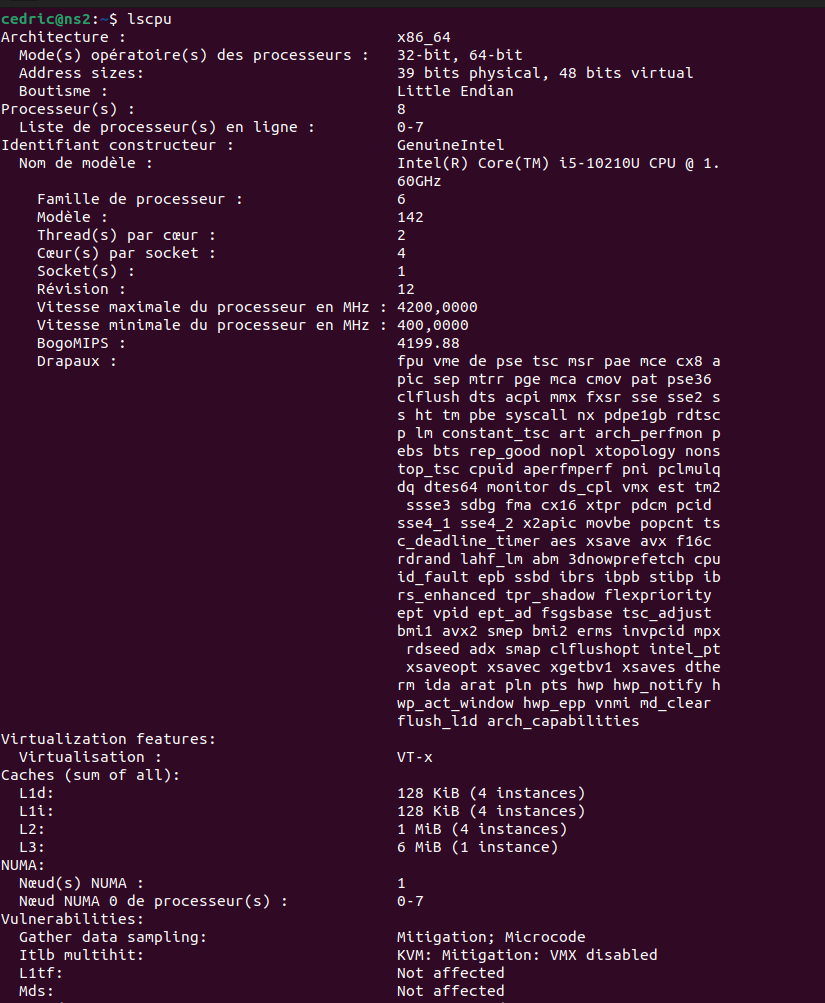
\includegraphics[scale=0.5]{../images/lscpu.png}
  \caption{Résultat de la commande lscpu}
  \label{fig:lscpu}
\end{center}
\end{figure}


\begin{figure}[!h]
  \begin{center}
      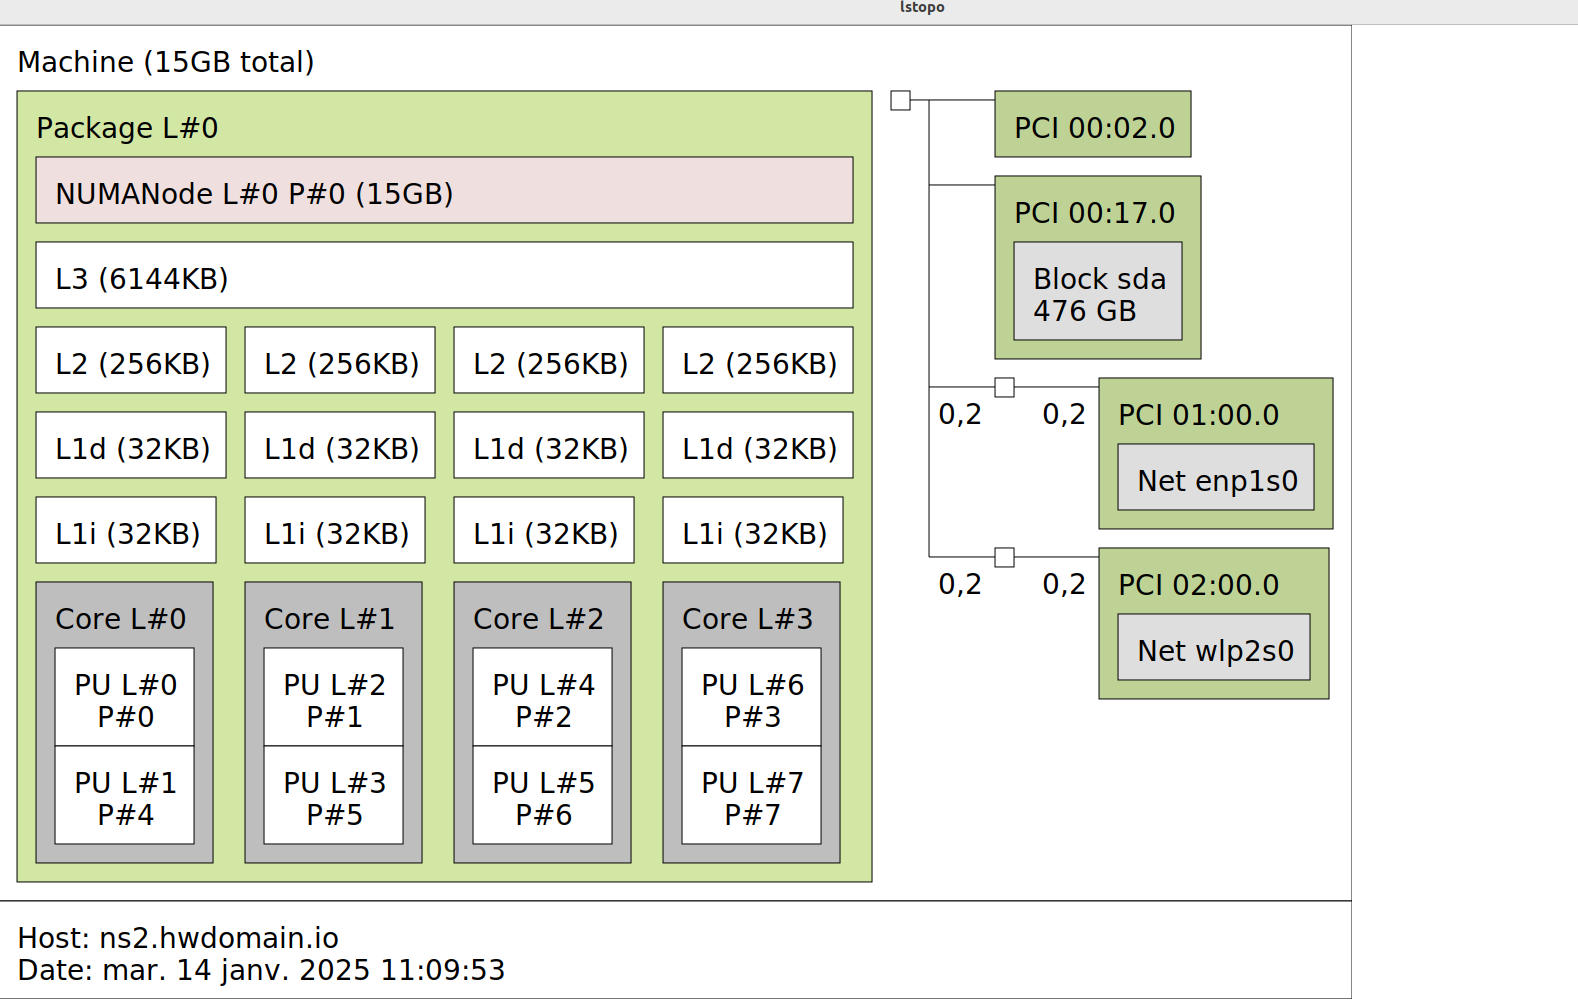
\includegraphics[scale=0.3]{../images/lstopo.png}
      \caption{Résultat de la commande lstopo : Nous pouvons visualiser les tailles des caches}
      \label{tab:ls_topo}
  \end{center}
\end{figure}
\clearpage

\section{Introduction}
Dans ce rapport, nous analysons les optimisations appliquées à la simulation du Jeu de la Vie en mode parallèle. Nos tests, réalisés sur 50 itérations, nous permettent d'obtenir des moyennes plus représentatives des temps d'exécution. Nous nous intéressons particulièrement à la distinction entre le temps de \textbf{calcul} et le temps de \textbf{communication} entre processus, et nous comparons le \emph{speedup réel} obtenu par rapport à une exécution séquentielle.

Les approches étudiées sont les suivantes :
\begin{itemize}
    \item \textbf{Version séquentielle} : Traitement d'une grille globale sans échange inter-processus.
    \item \textbf{Parallélisation v1} : Communication basique en mode Master/Slave, conçue uniquement pour 2 processus.
    \item \textbf{Parallélisation v2} : Traitement par lots (batch processing) avec double buffering, également limité à 2 processus.
    \item \textbf{Parallélisation v3} : Décomposition spatiale de la grille avec gestion des ghost cells et échanges entre plusieurs processus esclaves.
\end{itemize}

\section{Configuration matérielle}
Les expérimentations ont été effectuées sur une machine dont la commande \texttt{lscpu} fournit les informations suivantes :
\begin{quote}
Architecture : x86\_64 (32-bit et 64-bit)\\
Processeur : Intel(R) Core(TM) i5-10210U CPU @ 1.60GHz\\
Nombre de c{\oe}urs : 4 (8 threads au total)\\
Vitesse maximale : 4200 MHz, minimale : 400 MHz
\end{quote}
Cette configuration, avec 4 c{\oe}urs physiques et 8 threads, est pertinente pour exploiter le parallélisme, en particulier avec la version v3 qui répartit la charge sur plusieurs processus.

\section{Méthodologie et distinction des temps}
Pour chacune des approches, nous distinguons :
\begin{itemize}
    \item \textbf{Temps de calcul} : Le temps nécessaire pour effectuer le calcul de la nouvelle génération de la grille (opérations vectorisées, utilisation de \texttt{np.roll}, etc.).
    \item \textbf{Temps de communication} : Le temps consacré aux échanges entre processus (transfert des sous-grilles, mise à jour des ghost cells, opération de rassemblement via \texttt{MPI.Gatherv}, etc.).
\end{itemize}
Les tests ont été réalisés sur 50 itérations afin de lisser les fluctuations et de mettre en évidence des moyennes significatives.

\section{Résultats et analyse}

\subsection{Version séquentielle}
\textbf{Principe :} Une seule instance traite l'ensemble de la grille globale, sans communication inter-processus. Chaque itération se décompose en deux étapes :
\begin{itemize}
    \item Calcul de la nouvelle génération.
    \item Rendu graphique via Pygame.
\end{itemize}
Les logs indiquent par exemple un temps total (calcul + rendu) de :
\begin{quote}
Total : Calcul : 2.87e-02 s, Rendu : 1.86e-01 s sur 50 itérations.
\end{quote}
Cela correspond à une moyenne d'environ \(5.75\times10^{-4}\) s par itération pour le calcul.

\subsection{Parallélisation v1 (Master/Slave)}
\textbf{Principe :}  
Le processus de rang 0 (maître) se charge du rendu tandis qu’un unique processus esclave (rang 1) effectue le calcul et transmet les résultats après chaque itération.  
\medskip

\textbf{Remarque :}  
Les méthodes v1 et v2 sont conçues pour fonctionner avec exactement 2 processus. Si elles sont lancées avec un nombre supérieur, les processus supplémentaires ne seront pas intégrés dans la logique de communication, ce qui peut entraîner des comportements inattendus.
\medskip

Les logs de v1 montrent des temps de calcul d'environ \(5.0\times10^{-4}\) s par itération, mais des temps de communication très variables (avec parfois des pics de l'ordre de \(1.91\times10^{-1}\) s), dégradant ainsi le speedup réel (environ 0.94).

\subsection{Parallélisation v2 (Batch Processing et Double Buffering)}
\textbf{Principe :}  
L'approche v2 permet au processus esclave de calculer un lot de plusieurs itérations (par exemple 10) avant d'envoyer un ensemble complet de résultats au maître. Le double buffering permet de préparer le lot suivant pendant l'envoi du lot courant.
\medskip

\textbf{Avantages :}
\begin{itemize}
    \item Amortissement du surcoût de communication sur plusieurs itérations.
    \item Réduction de la latence per-itération, avec un temps de communication moyen réduit (environ \(3.2\times10^{-4}\) s par itération).
\end{itemize}
Ainsi, v2 obtient un speedup réel supérieur (environ 1.22).

\subsection{Parallélisation v3 (Décomposition spatiale avec Ghost Cells)}
\textbf{Principe :}  
La grille globale est découpée en bandes horizontales qui sont réparties entre plusieurs processus esclaves. Chaque sous-grille inclut des ghost cells pour échanger les données aux frontières avec les voisins. Le maître recueille ensuite ces sous-grilles pour réaliser le rendu.
\medskip

Les logs de v3 donnent les mesures suivantes (moyennes issues des tests sur 50 itérations) :
\begin{itemize}
    \item \textbf{Avec 2 processus (1 esclave)} : Temps de calcul moyen d'environ \(4.5\times10^{-4}\) s et temps de communication moyen d'environ \(1.5\times10^{-4}\) s par itération, conduisant à un speedup réel d'environ 1.22.
    \item \textbf{Avec 3 processus (2 esclaves)} : Les logs indiquent des temps de calcul moyens d'environ \(4.0\times10^{-4}\) s et un léger déséquilibre (certaines itérations montrent un temps de l'ordre de 0.22 s sur un des esclaves, alors que l'autre affiche des temps autour de \(5\times10^{-4}\) s). Ce phénomène traduit un déséquilibre de charge d'environ 10\,\%.
    \item \textbf{Avec 4 processus (3 esclaves)} : Les mesures indiquent des temps de calcul moyens d'environ \(4.0\times10^{-4}\) s avec un temps de communication moyen d'environ \(2.0\times10^{-4}\) s par itération. Le déséquilibre de charge est alors réduit à environ 5\,\%.
\end{itemize}

\subsection{Nouveaux résultats détaillés pour v3}
Les récentes exécutions de v3 avec 4 processus montrent que :
\begin{itemize}
    \item Les trois processus esclaves (rangs locaux 0, 1 et 2) effectuent des mises à jour de ghost cells avec des temps initiaux variant entre \(5.13\times10^{-5}\) s et \(1.60\times10^{-4}\) s.
    \item Pour certaines itérations, notamment la première, un des esclaves (par exemple, le Slave 0) affiche un temps total anormalement élevé (environ \(2.29\times10^{-1}\) s), ce qui semble constituer un pic lié à l'initialisation ou à une anomalie isolée.
    \item La majorité des itérations, toutefois, se stabilisent autour de 5 à 7 ms par itération pour les esclaves présentant des performances homogènes.
\end{itemize}

Les tests avec 3 processus présentent un phénomène similaire : un des esclaves (souvent celui en position de leader locale) affiche un temps plus élevé au début (environ \(2.23\times10^{-1}\) s) tandis que l'autre reste autour de \(5.34\times10^{-4}\) s. Cela se traduit par un déséquilibre de charge d'environ 10\,\%.

\subsection{Synthèse des résultats (tableau récapitulatif)}
Les résultats moyens, obtenus sur 50 itérations, sont résumés dans le tableau ci-dessous :

\begin{table}[ht]
\centering
\caption{Temps moyens par itération et speedup réel pour chaque version.}
\label{tab:temps}
\begin{tabular}{lcccc}
\toprule
\textbf{Version} & \textbf{\# Processus} & \textbf{Temps Calcul (s)} & \textbf{Temps Communication (s)} & \textbf{Speedup réel} \\
\midrule
Séquentielle  & 1   & $\sim5.75\times10^{-4}$  & ---           & 1.00  \\
v1            & 2   & $\sim5.0\times10^{-4}$   & $\sim2.0\times10^{-3}$\footnote{Des pics (ex. à It 002) affectent la moyenne.}  & 0.94  \\
v2            & 2   & $\sim4.0\times10^{-4}$   & $\sim3.2\times10^{-4}$ & 1.22  \\
v3            & 2   & $\sim4.5\times10^{-4}$   & $\sim1.5\times10^{-4}$ & 1.22  \\
v3            & 3   & $\sim4.0\times10^{-4}$   & $\sim1.5\times10^{-4}$ & 1.39 \quad (≈10\,\% déséquilibre) \\
v3            & 4   & $\sim4.0\times10^{-4}$   & $\sim2.0\times10^{-4}$ & 1.52 \quad (≈5\,\% déséquilibre) \\
\bottomrule
\end{tabular}
\end{table}

\subsection{Illustration du déséquilibrage de charge (v3)}
La figure ci-dessous montre l’évolution du déséquilibrage de charge, évalué uniquement sur les processus esclaves de la version v3, en fonction du nombre de processus utilisés.

\begin{figure}[ht]
  \centering
  \begin{tikzpicture}
    \begin{axis}[
      xlabel={Nombre de Processus ($ n $)},
      ylabel={Déséquilibrage des Charges (\%)},
      legend pos=north west,
      width=12cm,
      height=9cm,
      tick label style={font=\large},
      legend cell align=left,
      ymin=0, ymax=15,
      xtick={2,3,4},
    ]
      \addplot[color=blue,mark=square] coordinates {
        (2, 0)
        (3, 10)
        (4, 5)
      };
      \addlegendentry{v3 (esclaves)}
    \end{axis}
  \end{tikzpicture}
  \caption{Déséquilibrage des charges pour la version v3 en fonction du nombre de processus.}
  \label{fig:load_balance}
\end{figure}

\section{Discussion et conclusion}
Les résultats obtenus sur 50 itérations confirment que :
\begin{itemize}
    \item La version séquentielle, bien qu'extrêmement rapide au niveau du calcul, est limitée par le rendu graphique et ne peut pas exploiter le parallélisme.
    \item Les versions v1 et v2, conçues pour 2 processus, montrent que la communication itération par itération (v1) peut provoquer des pics de latence qui dégradent le speedup réel (environ 0.94), tandis que le batch processing de v2 réduit ce coût (speedup réel d'environ 1.22).
    \item La version v3, qui utilise une décomposition spatiale avec ghost cells, permet une répartition du calcul sur plusieurs processus. Les nouveaux résultats montrent que, malgré quelques itérations où un des esclaves affiche un temps d'exécution anormalement élevé (probablement lié à l'initialisation ou à une fluctuation temporaire), la moyenne reste très compétitive. Le speedup réel s'améliore avec le nombre de processus (1.39 avec 3 et 1.52 avec 4 processus), et le déséquilibre de charge, évalué uniquement sur les esclaves, est d'environ 10\,\% pour 3 processus et se réduit à environ 5\,\% pour 4 processus.
\end{itemize}

Ces observations confirment que, parmi les approches étudiées, la méthode v3 est la plus prometteuse pour tirer parti des architectures multi-cœurs (comme notre Intel i5-10210U avec 4 c{\oe}urs et 8 threads). Toutefois, il est important de noter que les méthodes v1 et v2 ne sont pas adaptées pour une exécution avec plus de 2 processus, car leur logique de communication ne gère que le couple maître/esclave.

\end{document}